\documentclass[border=10pt]{standalone}
\usepackage{pgfplots}
\pgfplotsset{compat=1.18}
\begin{document}
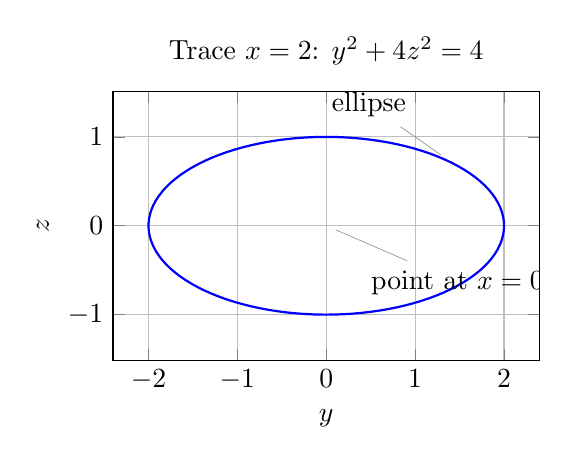
\begin{tikzpicture}
\begin{axis}[
    title={Trace $x=2$: $y^2+4z^2=4$},
    xlabel={$y$}, ylabel={$z$},
    axis equal,
    grid=both,
    width=7cm,
    height=5cm,
    xmin=-2.4, xmax=2.4,
    ymin=-1.2, ymax=1.2,
]
\addplot[domain=0:360, samples=120, blue, thick]
({2*cos(x)}, {sin(x)});
\node[pin=above left:{ellipse}] at (axis cs:1.4,0.72) {};
\node[pin=below right:{point at $x=0$}] at (axis cs:0,0) {};
\end{axis}
\end{tikzpicture}

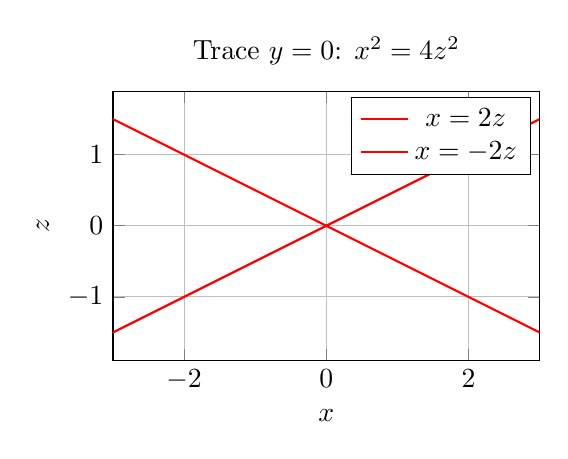
\begin{tikzpicture}
\begin{axis}[
    title={Trace $y=0$: $x^2=4z^2$},
    xlabel={$x$}, ylabel={$z$},
    axis equal,
    grid=both,
    width=7cm,
    height=5cm,
    xmin=-3, xmax=3,
    ymin=-1.5, ymax=1.5,
]
\addplot[domain=-3:3, red, thick] {0.5*x};
\addplot[domain=-3:3, red, thick] {-0.5*x};
\addlegendentry{$x=2z$};
\addlegendentry{$x=-2z$};
\end{axis}
\end{tikzpicture}
\end{document}